\section{Empirical Evaluation}
%- resultados basicos segun los distintos encodings
%- resultados comparativos de cuando empiezan a fallar en mapas cuadrados vacios
%- analisis varios (porq el encoding mejora o empeora)
%- hablar de cosas negativas
%- empezar a ver una cota tentativa segun numero de celdas.

%- comparar cambiar restricciones del dijkstra. Un problema en grilla cuadrada.
%- usar la version mas simple.


We compared our algorithm to publicly available search-based solvers as well as MDD-SAT \cite{Surynek14} (enc=mdd), on congested grids. We ran two state-of-the-art search algorithms:  EPEA* \cite{Goldenberg14}, and ICBS-h \cite{FelnerLB00KK18}.

The code used for our implementation was written in Python 3.7 using Clingo 5.3 () for the ASP solver. Clingo was run with 4 threads in \textit{parallel-mode}, and using \textit{usc} as the optimization strategy. The search based algorithms use a implementation written C\#, based on the implementation in \cite{FelnerLB00KK18}. The MDD-SAT algorithm use a implementation written C++ based in (cita de surynek)

All the experiments were tested on a 3.40GHz Intel Core i5-3570K computer with 8GB of memory. We set a runtime limit of 5 minutes for all the problems.

\subsection{Open $N$ x $N$ grids experiments} First, we experimented on different empty grids (No obstacles), with sizes $N=\{8,16,32,64\}$. For each one of these grids we generated $10$ instances
for each number of agents between $A=\{2,4, \ldots N^2 -2 \}$. All the agents initial positions and goals were randomly placed. We compared different encodings, where ASP-basic is a basic encoding that uses quadratic conflict resolution and grid dependent penalties. ASP-indep uses quadratic conflict resolution and grid independent penalties. Finally, ASP-lin-indep uses linear conflict resolution and grid independent penalties.


In figure we show the \emph{breaking point}. of the thingy


\subsection{N x N grids with random obstacles experiments} 
Next, we experimented on $8\times 8$ and $20\times 20$ randomly generated problems with 10\% obstacles. For $8\times8$ (resp.~$20\times 20$) we generate 150 (resp.~160) problems with the number of agents in $\{4,\dots,18\}$ (resp.~$\{20,22,\ldots,50\}$). Success rates, and number of problems solved versus time are shown in Figure ~\ref{fig_obs}. 

analisis


\subsection{Warehouse experiments}
Also, we experimented on a the warehouse grid shown in Figure ~\ref{fig_ware} . 

analisis




\begin{figure*}
    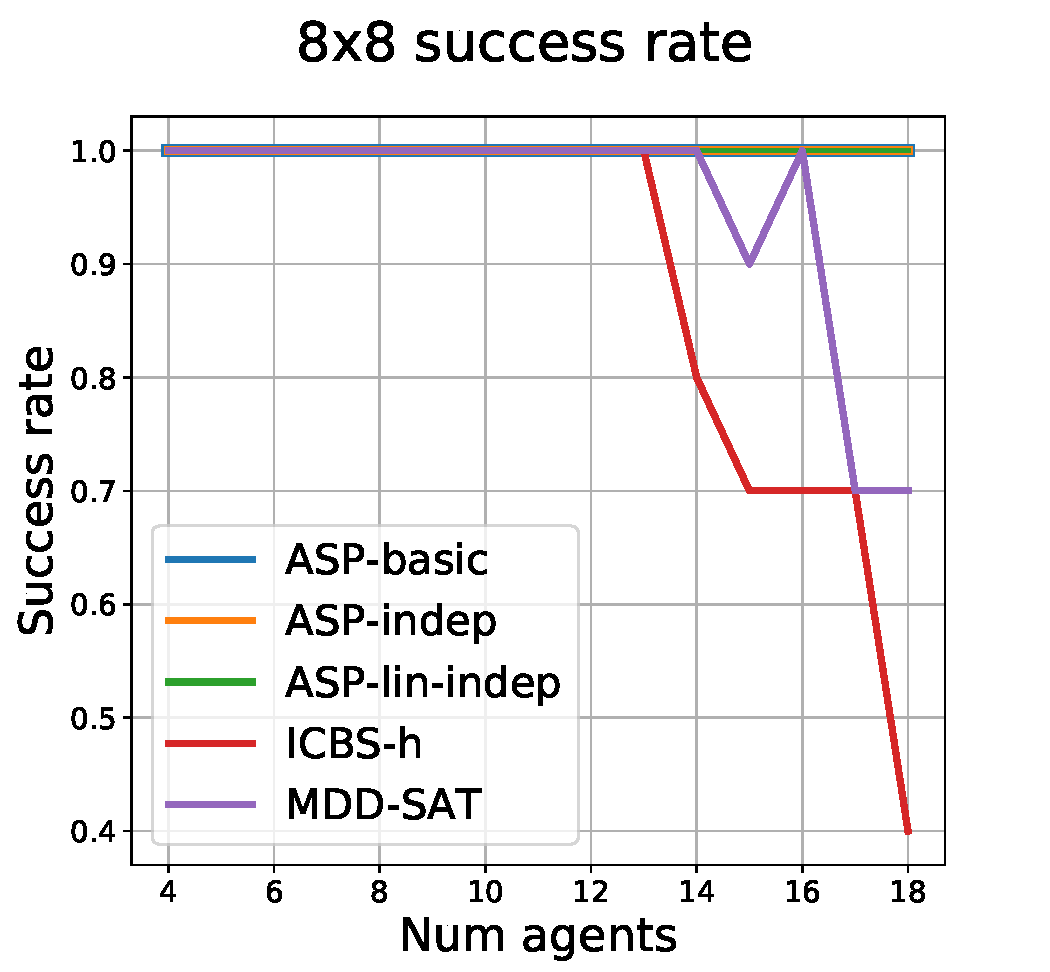
\includegraphics[width=0.24\textwidth]{graphs/8x8succ.pdf}
    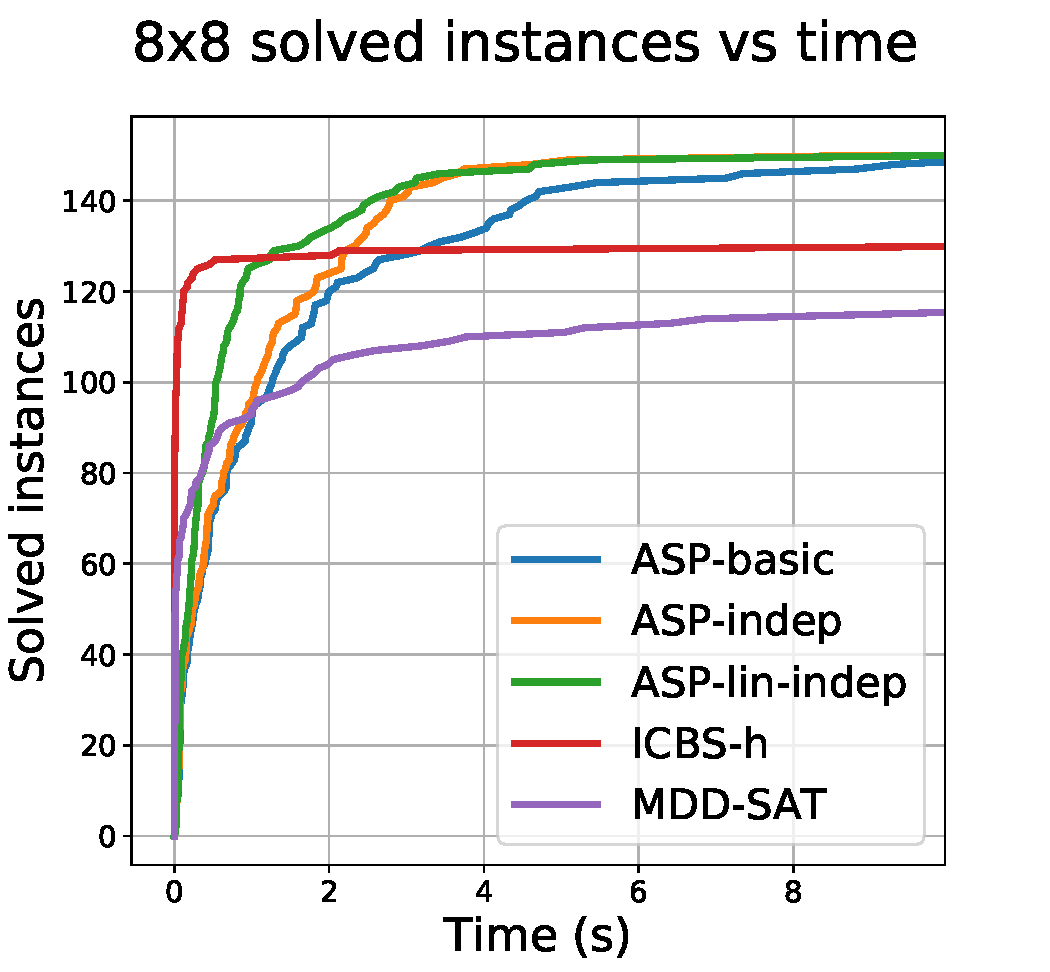
\includegraphics[width=0.24\textwidth]{graphs/8x8runtime.pdf}
    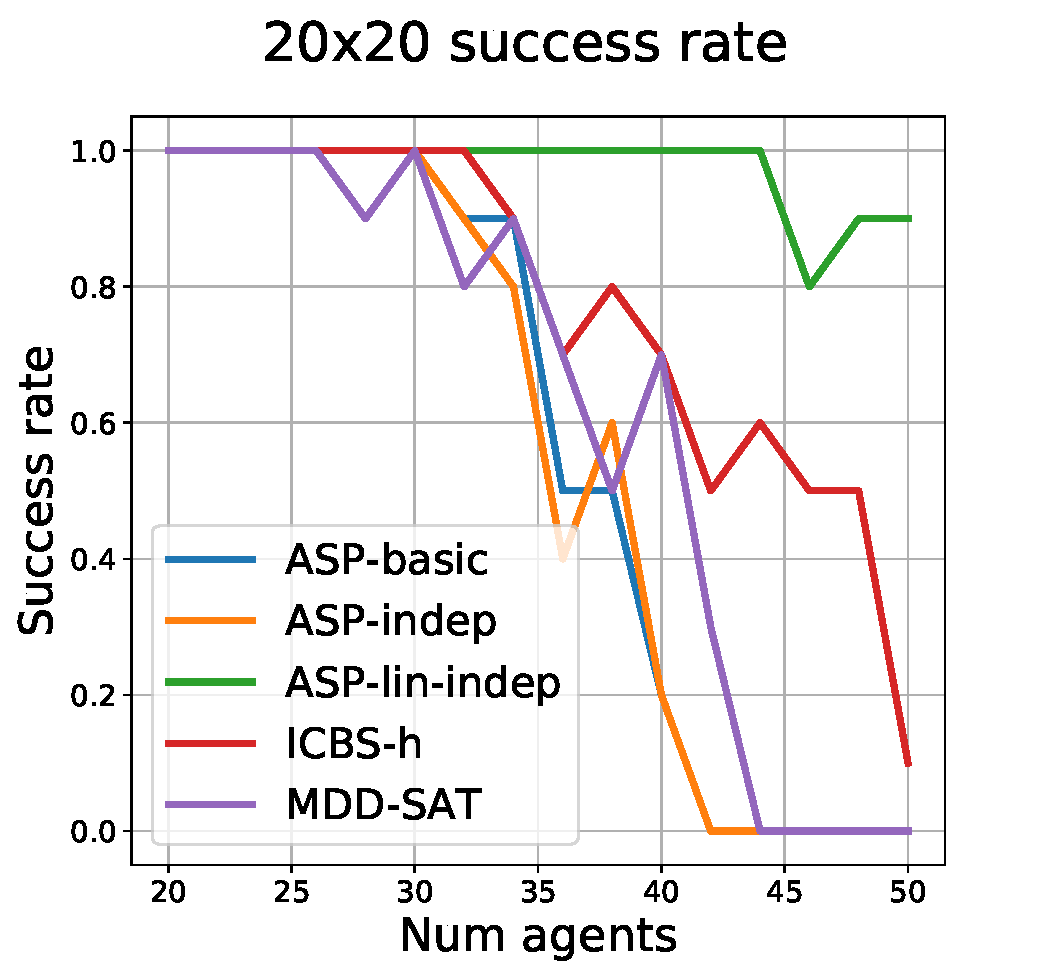
\includegraphics[width=0.24\textwidth]{graphs/20x20succ.pdf}
    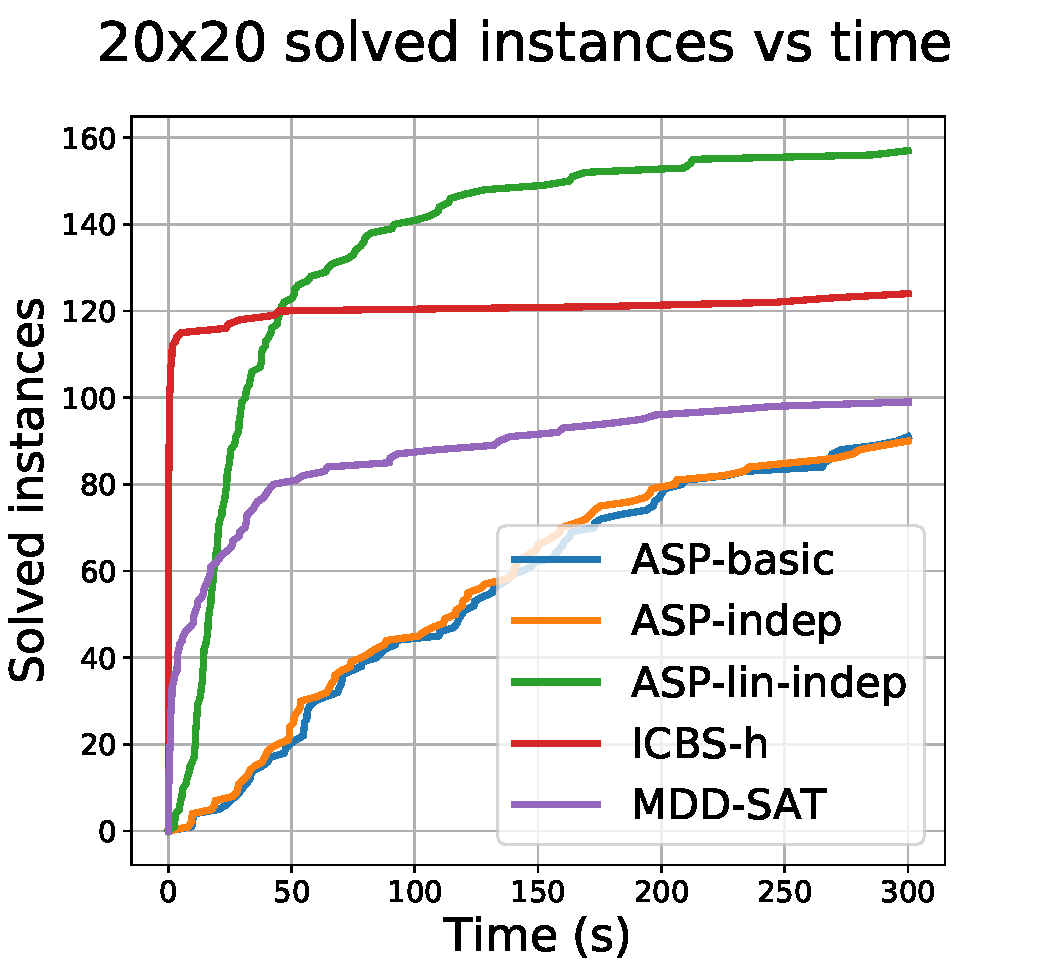
\includegraphics[width=0.24\textwidth]{graphs/20x20runtime.pdf}
    \caption{Success rate and number of instances solved versus time on $8\times 8$ and $20\times 20$ grids.}
    
    \label{fig_obs}
\end{figure*}

\begin{figure*}
    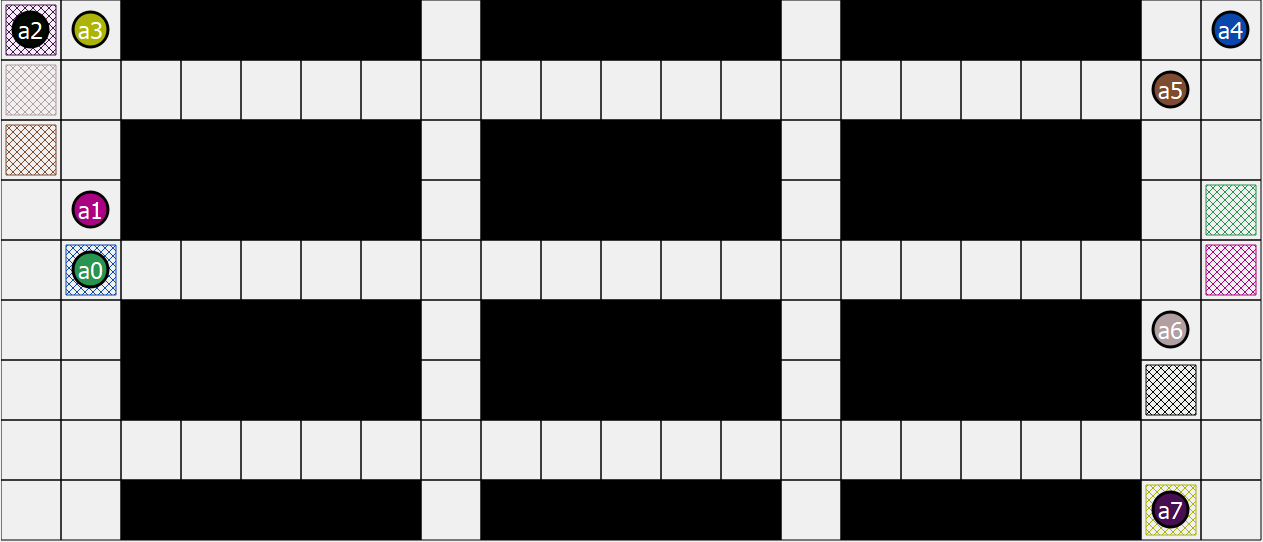
\includegraphics[width=0.45\textwidth]{graphs/warehouse.PNG}
    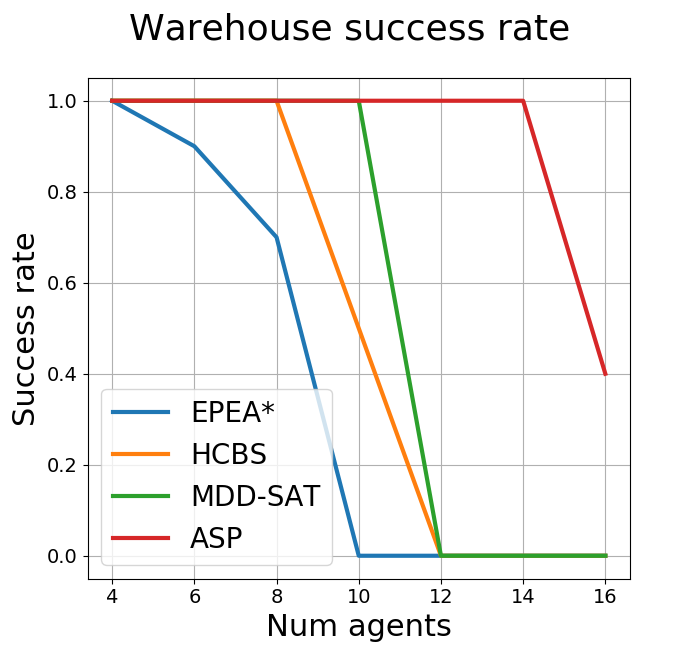
\includegraphics[width=0.24\textwidth]{graphs/warehousesucc.png}
    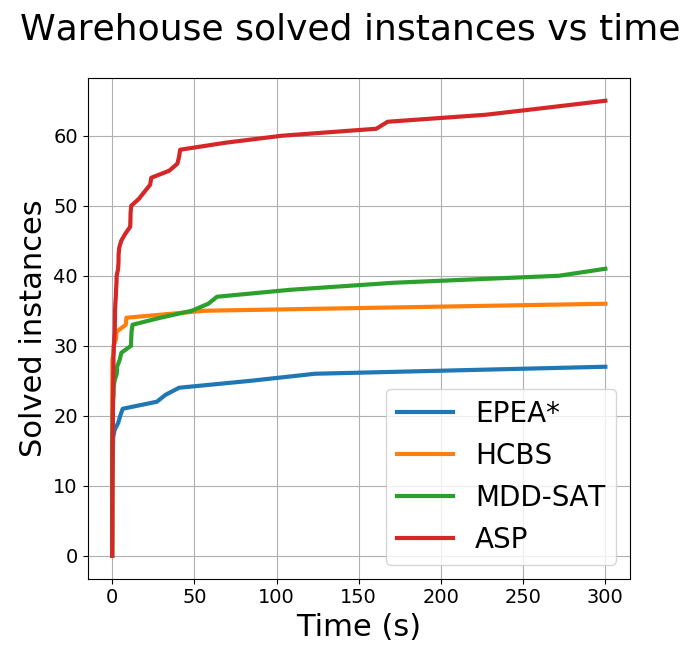
\includegraphics[width=0.24\textwidth]{graphs/warehouseruntime.png}
    \caption{Warehouse problem example and results}
    \label{fig_ware}
\end{figure*}

